\chapter{Система на кристалле}

Система на кристалле  (SoC,  СНК)  — это функционально законченная электронная вычислительная система, состоящая из одного или нескольких микропроцессорных модулей,а также системных и периферийных контроллеров, выполненная на одном кристалле.

Рассмотрим функциональную схему разрабатываемой системы на кристалле, которая показана на рисунке \ref{img:scheme}.

\begin{figure}[H]
	\begin{center}
		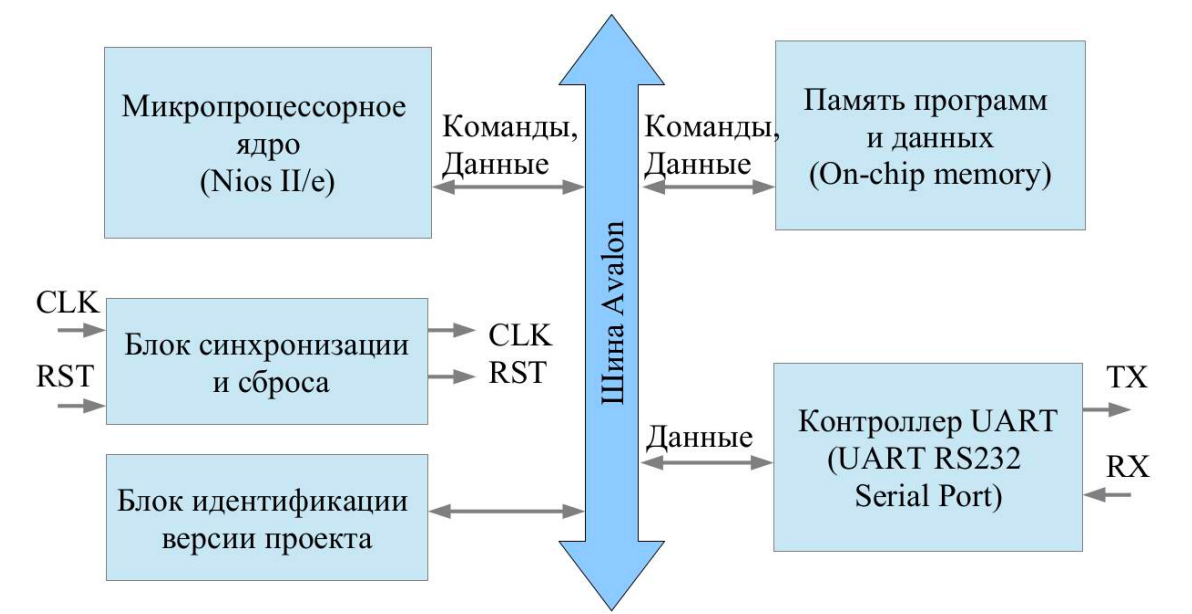
\includegraphics[scale=0.3]{img/scheme.png}
	\end{center}
	\captionsetup{justification=centering}
	\caption{Функциональная схема разрабатываемой системы на кристалле}
	\label{img:scheme}
\end{figure}

Система на кристалле состоит из следующих блоков:
\begin{itemize}
	\item микропроцессорное ядро Nios II/e выполняет функции управления системой;
	\item внутренняя оперативная память СНК, используемая для хранения программы управления и данных;
	\item системная шина Avalon обеспечивает связность всех компонентов системы;
	\item блок синхронизации и сброса обеспечивает обработку входных сигналов сброса и синхронизации и распределение их в системе. Внутренний сигнал сброса синхронизирован и имеет необходимую для системы длительность;
	\item блок идентификации версии проекта обеспечивает хранение и выдачу уникального идентификатора версии, который используется программой управления при инициализации системы;
	\item контроллер UART обеспечивает прием и передачу информации по интерфейсу RS232.
\end{itemize}

\chapter{Проектирование системы}

Проектирование выполнялось на системе автоматизированного проектирования (САПР) Altera Quartus II.

На рисунке \ref{img:module} представлен модуль системы на кристалле Altera Qsys, построенный на основе функциональной схемы \ref{img:scheme}.

\begin{figure}[H]
	\begin{center}
		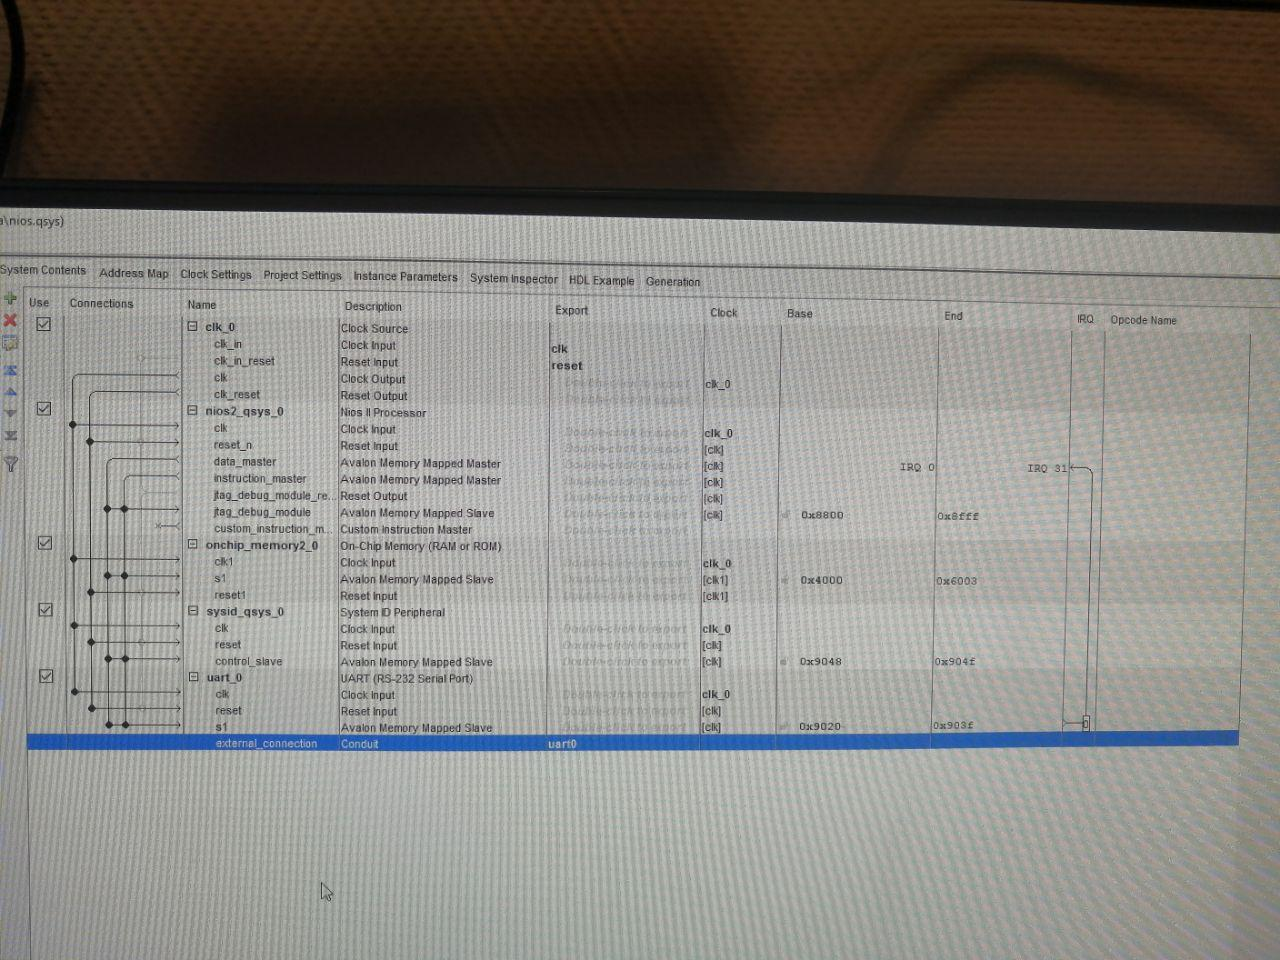
\includegraphics[scale=1.0]{img/module.jpg}
	\end{center}
	\captionsetup{justification=centering}
	\caption{Готовый модуль в системе проектирования систем на кристалле Altera Qsys}
	\label{img:module}
\end{figure}

САПР Quartus II автоматически выделяет каждому подключенному компоненту свое собственное адресное пространство, которое едино для данных и кода по принципу Фон Неймана. Корректное распределение необходимо во избежание возникновения ошибок. На рисунке \ref{img:map} представлена таблица распределения адресов, которая была автоматически получена для данной системы.

\begin{figure}[H]
	\begin{center}
		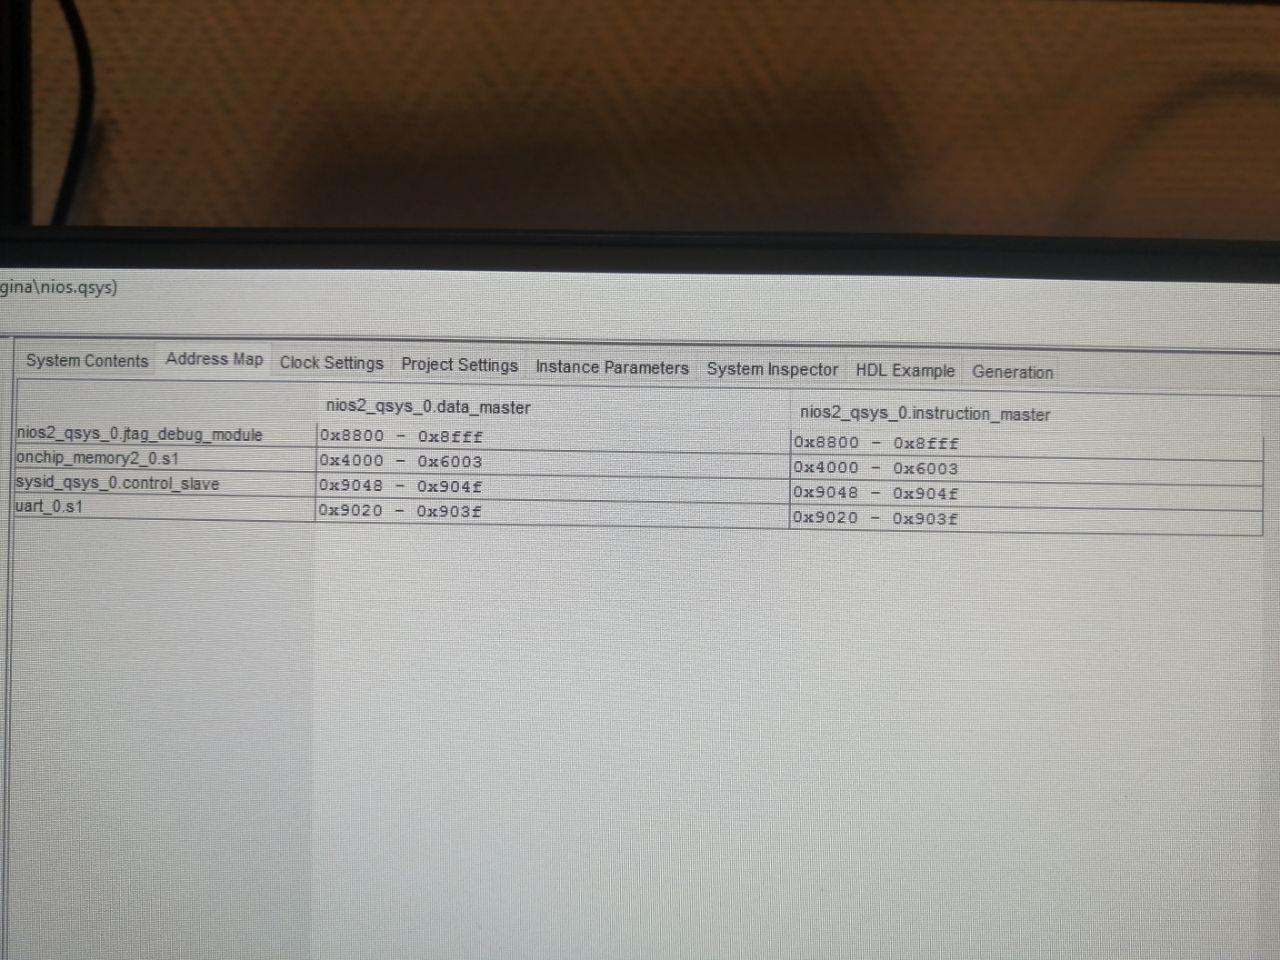
\includegraphics[scale=0.9]{img/map.jpg}
	\end{center}
	\captionsetup{justification=centering}
	\caption{Таблица распределения адресов}
	\label{img:map}
\end{figure}

Назначение портам проекта контактов микросхемы показано на рисунке \ref{img:planner}.

\begin{figure}[H]
	\begin{center}
		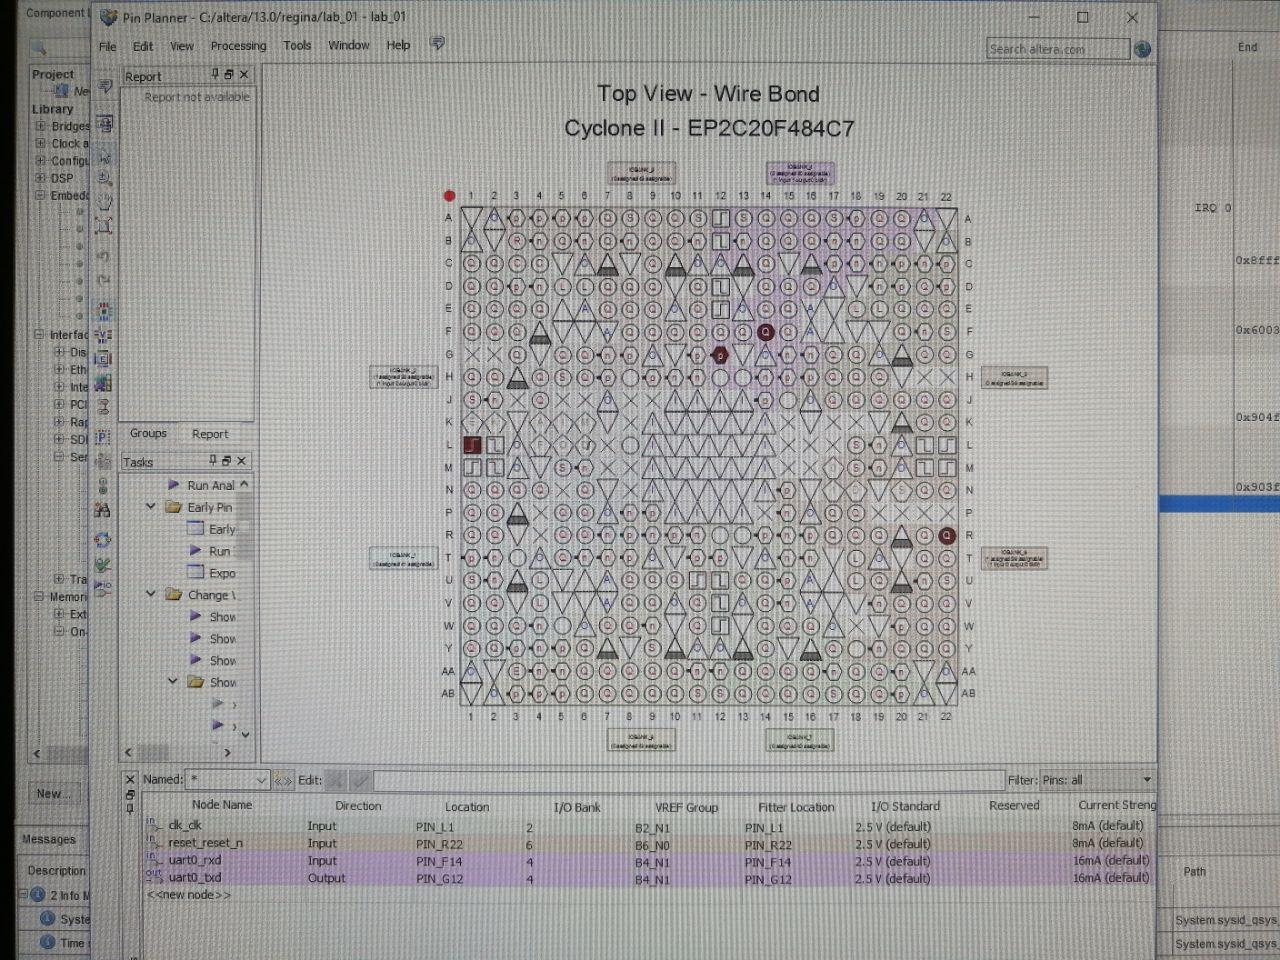
\includegraphics[scale=0.9]{img/planner.jpg}
	\end{center}
	\captionsetup{justification=centering}
	\caption{Назначение портам проекта контактов микросхемы}
	\label{img:planner}
\end{figure}

\chapter{Верификация системы}

Верификация системы проводилась с использованием программы терминала.

Код, представленный на рисунке \ref{img:code},  передает по UART значение SystemID (32-х разрядный код, состоящий из номера группы и варианта) в виде четырех байт символов в ASCII формате. Параметр SystemID был ранее задан значением "5313".

\begin{figure}[H]
	\begin{center}
		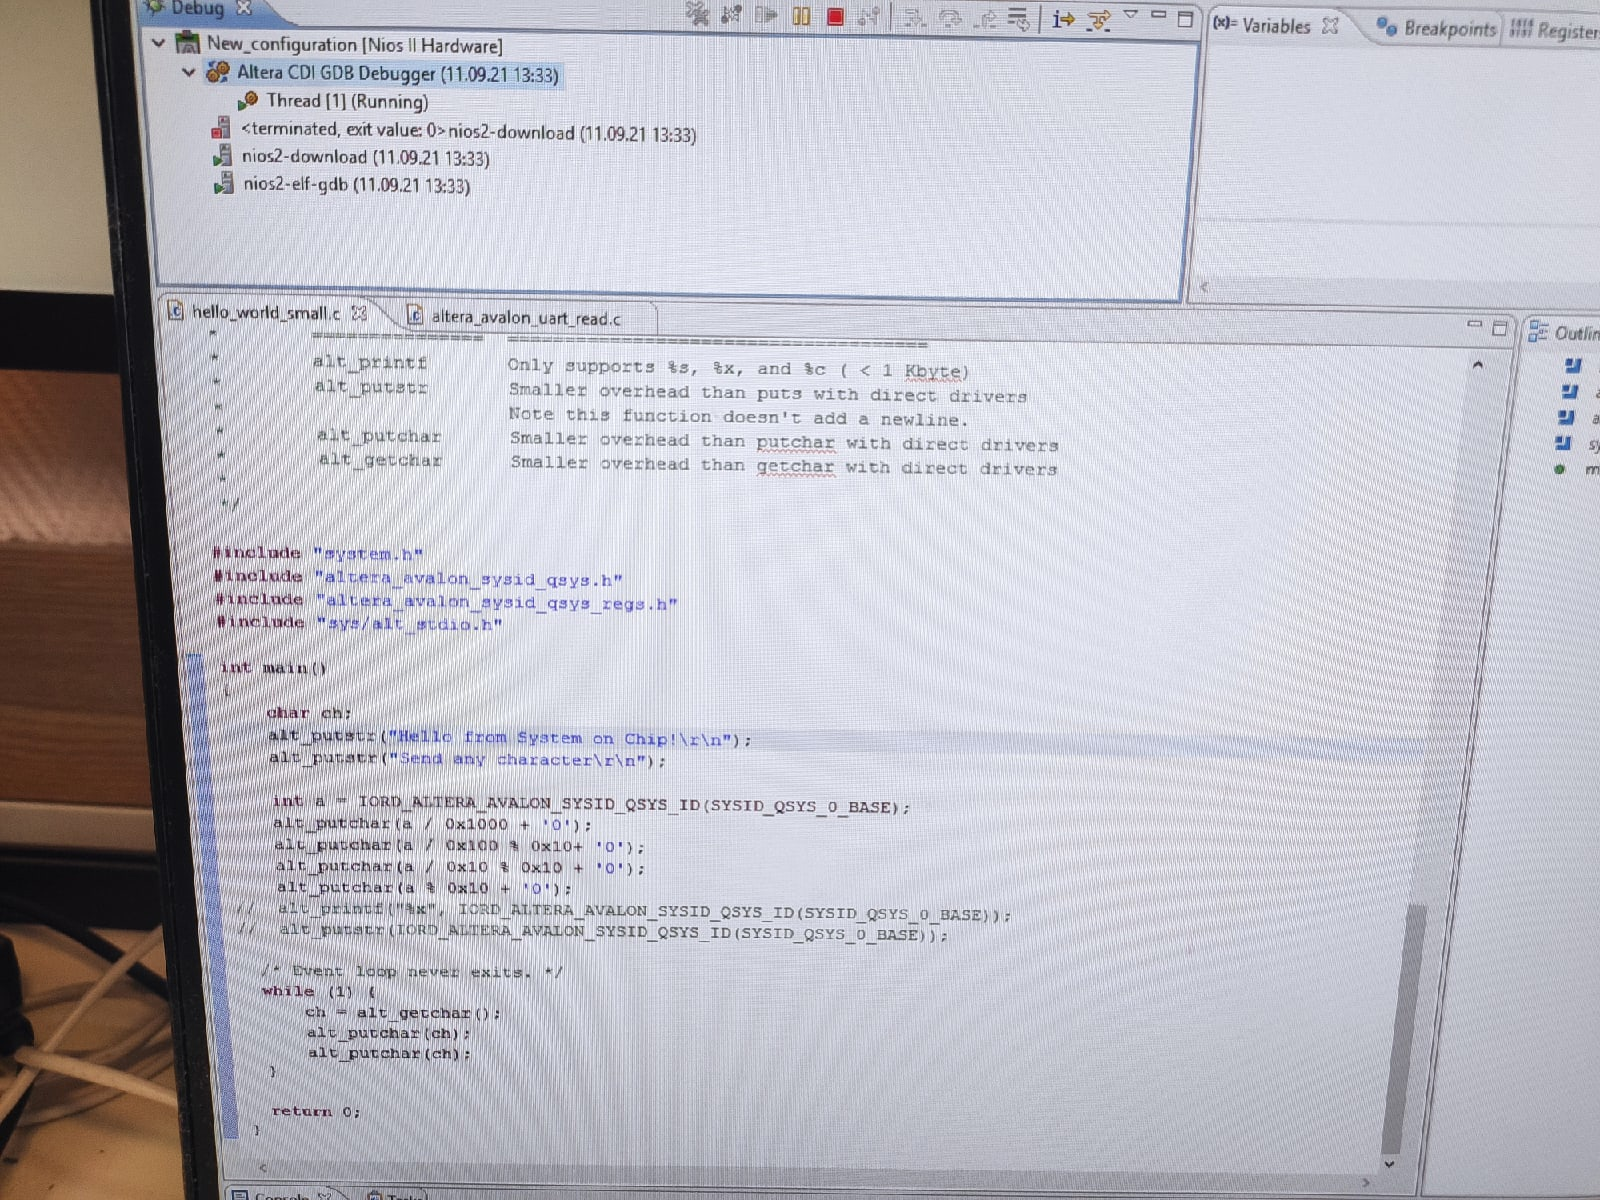
\includegraphics[scale=0.3]{img/code.jpg}
	\end{center}
	\captionsetup{justification=centering}
	\caption{Код программы микропроцессорного ядра NIOS2}
	\label{img:code}
\end{figure}

Вывод SystemID на экран показан на рисунке \ref{img:result}.

\begin{figure}[H]
	\begin{center}
		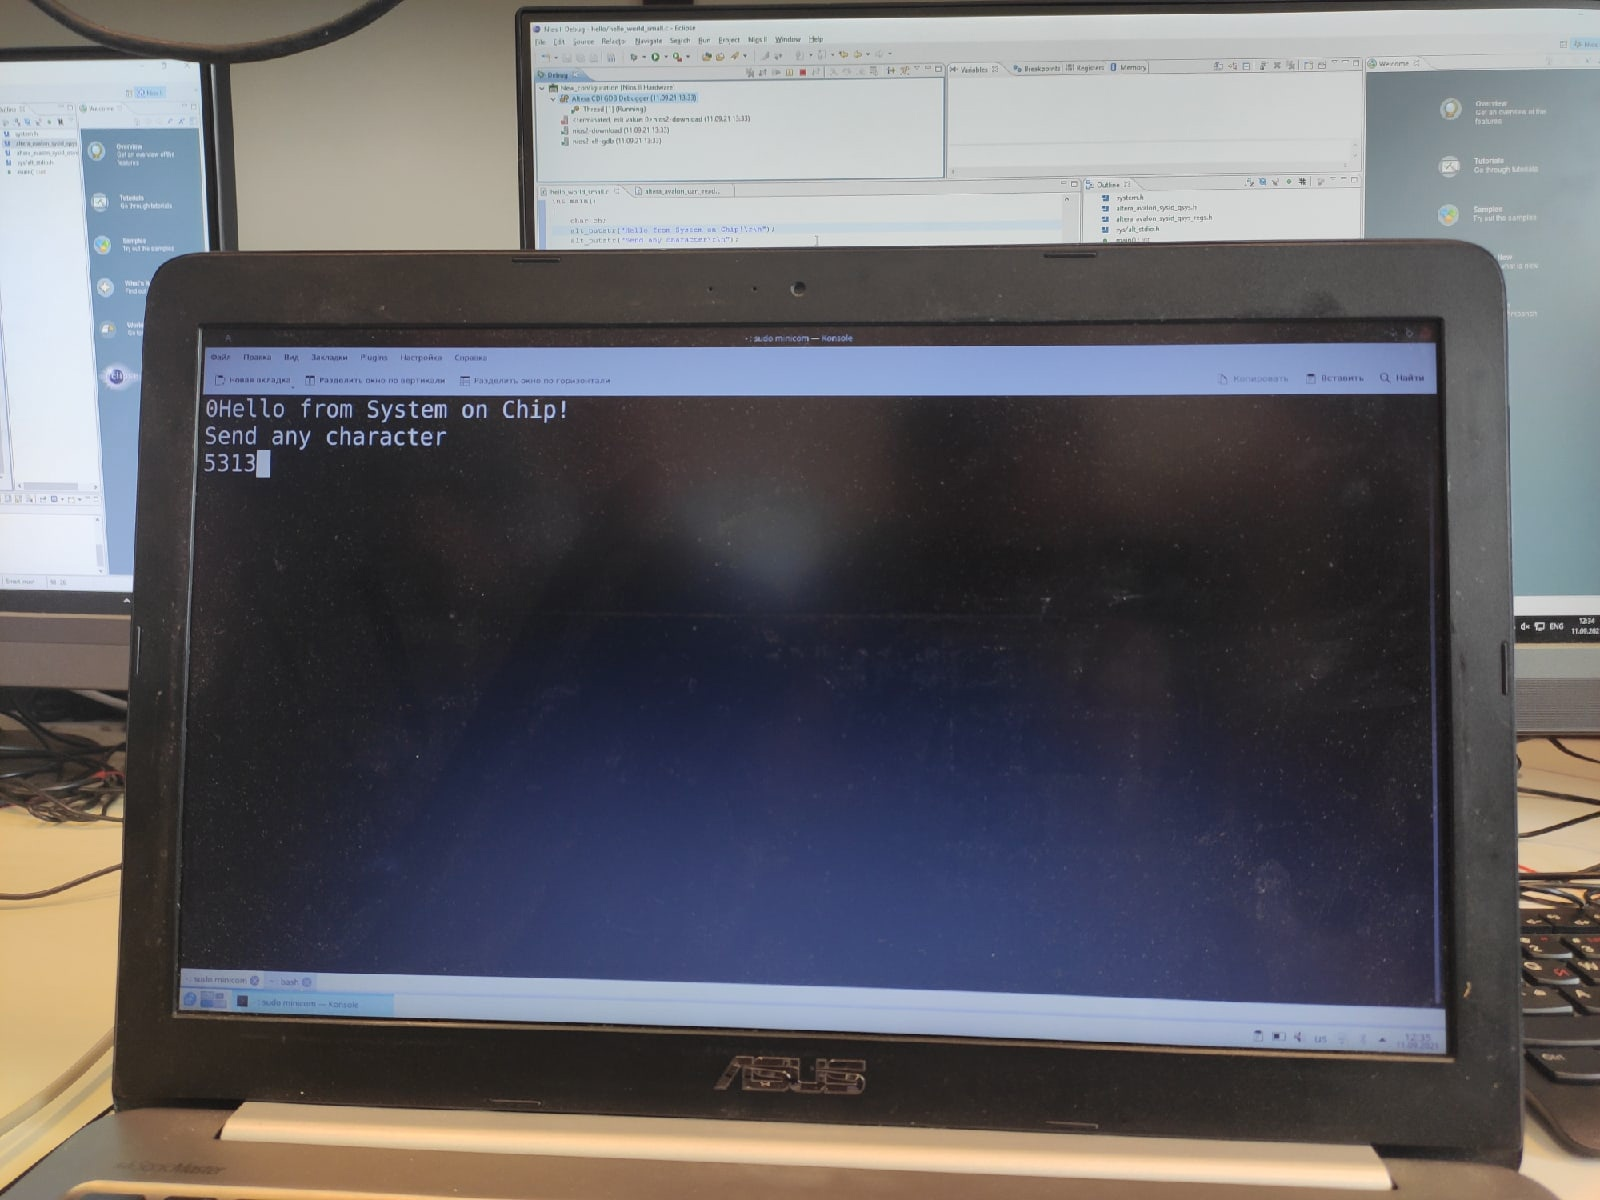
\includegraphics[scale=0.3]{img/result.jpg}
	\end{center}
	\captionsetup{justification=centering}
	\caption{Верификация проекта с использованием программы терминала}
	\label{img:result}
\end{figure}

\textit{Примечание:} в связи с наличием одной отладочной платы, верификация проводилась на программе одногруппника, которую было разрешено прикладывать в отчете.

  


